\vspace{-3cm}\chapter{实验1. UPC码}

\section{1.1 题目}
UPC码由12个数字构成,其中最右侧的数字是校验位,我们用 d1 表示,那么 UPC 码经过下面的公式计算之后必须是 10 的倍数
$$
\left(d_{1}+d_{3}+d_{5}+d_{7}+d_{9}+d_{11}\right)+3\left(d_{2}+d_{4}+d_{6}+d_{8}+d_{10}+d_{12}\right).
$$
比如,0-48500-00102 的校验位就是 8,因为经过上面的公式计算之后,只有数字 8 才可以得到 10 的倍数值 50
$$
(\mathbf{\color{red}8}+0+0+0+5+4)+3(2+1+0+0+8+0)=50.
$$

编写一个程序,通过命令行参数方式\textbf{输入1个11位的数字},\textbf{输出一个完整的12位}的UPC码。注意:
\begin{enumerate}
    \item 11 位数字可以包含前导零;
    \item 11 位数字的大小已经使得数字的表示范围超过了 \lstinline{int} 类型能够表示的大小了;
    \item 如果不要求用户严格的输入11位的数字,那么就需要在真正执行计算之前对用户输入的参数合法性进行考虑,
        请问你能列举出有多少种不合法的输入出现呢?如果程序的健壮性足够好,那就必须能处理这些意外的输入。
\end{enumerate}

\section{1.2 题目分析}

本题目共分为三部分:
\begin{enumerate}
    \item \textbf{数据的输入}. 本题中数据是通过命令行输入的11位数字,也就是以String的形式存储在\lstinline{args[0]}中,
        Java中String类的丰富method可以帮助我们把String当作数组来处理。
    \item \textbf{异常数据的检测}. 本题中可能出现三种异常数据:输入参数个数错误,长度不为11,字符串有非数字符,校验位结果错误。
    \begin{itemize}
        \item 输入参数个数错误可以通过\lstinline{args.length}判断
        \item 长度可以通过\lstinline{args[0].length()}判断
        \item 字符串的非字符数组在扫描数组过程中通过\lstinline{Character.isDigit()}判断
        \item 校验位结果错误可以在计算完成后判断
    \end{itemize}
    \item \textbf{算法设计}. 观察UPC码的计算方法不难发现,UPC码校验位的计算即用50减去三倍的偶位数和一倍的奇位数。
        将本题输入数据看作数组\lstinline{s},则\lstinline{s[0]} = $d_{2}$,所以数组索引的奇偶和UPC码的奇偶相同。 
    \item \textbf{代码说明}. 依据前三条的思路构建代码如下
    \lstinputlisting[
        language = Java,
        caption = {\bf Problem1.java}    
    ]{../../../ProblemSet/src/Problem1.java}
\end{enumerate}

\section{1.3 数据设计}

本体主要目的为计算和检验异常数据,所以提供两个成功数据和几个对应于异常数据原因的数据得到验证即可。
为了便于对比输入输出,将每一次的输出打印出来
具体数据如下
\begin{table}[H]
    \centering
    \begin{tabular}{|c|c|c|c|}
    \hline
    \textbf{Input} & \textbf{Output} & \textbf{Input} & \textbf{Output} \\ \hline
    04850000102    & 804850000102    & 04850000103    & 504850000103    \\ \hline
    04850000100    & $d_0$ error(14)        & 04850000109    & $d_0$ error(-13)        \\ \hline
    1              & length error    & 012345678900   & length error    \\ \hline
    0123456a789    & not num         & 01?23456789    & not num         \\ \hline
    04850000102 1 & argu num error  &   & \\ \hline
    \end{tabular}
\end{table}

\section{1.4 结果展示}

\begin{figure}[H]
	\centering
	\begin{subfigure}{0.325\linewidth}
		\centering
		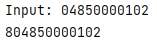
\includegraphics[width=0.7\linewidth]{../pic/1/1.1.png}
	\end{subfigure}
	\begin{subfigure}{0.325\linewidth}
		\centering
		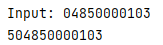
\includegraphics[width=0.7\linewidth]{../pic/1/1.2.png}
	\end{subfigure}
	\begin{subfigure}{0.325\linewidth}
		\centering
		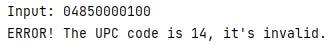
\includegraphics[width=1\linewidth]{../pic/1/1.3.png}
	\end{subfigure}
    \vspace{1cm}
    \begin{subfigure}{0.325\linewidth}
		\centering
		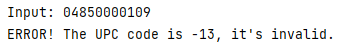
\includegraphics[width=1\linewidth]{../pic/1/1.4.png}
	\end{subfigure}
	\begin{subfigure}{0.325\linewidth}
		\centering
		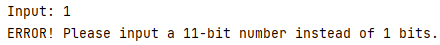
\includegraphics[width=1\linewidth]{../pic/1/1.5.png}
	\end{subfigure}
	\begin{subfigure}{0.325\linewidth}
		\centering
		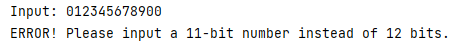
\includegraphics[width=1\linewidth]{../pic/1/1.6.png}
	\end{subfigure}
    \vspace{1cm}
    \begin{subfigure}{0.325\linewidth}
		\centering
		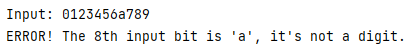
\includegraphics[width=1\linewidth]{../pic/1/1.7.png}
	\end{subfigure}
	\begin{subfigure}{0.325\linewidth}
		\centering
		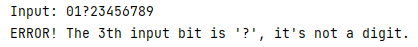
\includegraphics[width=1\linewidth]{../pic/1/1.8.png}
	\end{subfigure}
	\begin{subfigure}{0.325\linewidth}
		\centering
		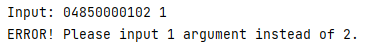
\includegraphics[width=1\linewidth]{../pic/1/1.9.png}
	\end{subfigure}
	\caption{Output of Problem1}
\end{figure}

\section{1.6 总结与收获}

本题比较简单,总结收获如下:
\begin{itemize}
    \item 对字符串的处理中可以使用丰富的Java库函数,让人大开眼界;
    \item 对程序健壮性的测试需要考虑很多可能,有多种违规输入,同时为了提高实用性也应该为不同的违规输入定制错误提醒;
    \item 由于违规输入较多,测试时如果采用Junit测试效果更好,可惜我被Junit5的配置折腾得快崩溃了,希望以后能再找机会学习。
\end{itemize}


% 1、题目
% 2、数据设计
% 3、算法设计
% 4、主干代码说明
% 5、运行结果展示
% 6、总结和收获